\documentclass[14pt]{extarticle}
\usepackage{amsmath}
\usepackage{amssymb}
\usepackage{graphicx}
\graphicspath{ {../chap10/} }
\usepackage[top=1in, bottom=0.75in, left=0.75in, right=0.75in]{geometry}
\newcommand*{\Scale}[2][4]{\scalebox{#1}{\ensuremath{#2}}}%
\usepackage{hyperref}
\usepackage[most]{tcolorbox}
\definecolor{bg}{RGB}{255,249,227}


\begin{document}

\section*{Math 208 Discussion Outline for 11/24/2020}


\subsection{Homework and other due dates}
\begin{itemize}

\item Section 10.1 due 11/24
\item Section 10.2 due 12/01
\item I recommend reading 10.3 and 10.4 and attempting the homework.
\end{itemize}

\subsection{Going Virtual}

\subsection{Questions?}

\subsection{Section 10.1: e}
\subsubsection*{Goals}
\begin{itemize}
	\item Recall and understand basics of $e$
	\item Solve continuous compounding questions
\end{itemize}
\subsubsection*{Detail}
One  of the most important numbers in math is $e$. You will come across it often, it is very useful, and it has some very interesting properties.
\begin{align*}
	&e = \lim_{n \to \infty} \left(1 + \frac{1}{n}\right)^n &
	\textbf{ or } &
	&e = \lim_{s \to 0} \left(1 + s\right)^{\frac{1}{s}}
\end{align*}
It is often used for modeling continuous growth. It is the base for the natural logarithm and an its slope is equal to its value.
\begin{align*}
	\frac{d}{dx}e^x =  e^x
\end{align*}
Some additional properties:
\begin{align*}
	&e^0 = 1 & &e^{x+y} = e^x e^y & &e^{-x}=\frac{1}{e^x} \\
	&e^{x-y} = \frac{e^x}{e^y }	& &(e^x)^r= e^{rx} & &\ln(e^x) = x
\end{align*}

\cleardoublepage
We have already seen it used in continuous compounding, where:
\begin{align*}
	A = Pe^{rt}
\end{align*}

\subsubsection*{Examples}
\begin{center}
	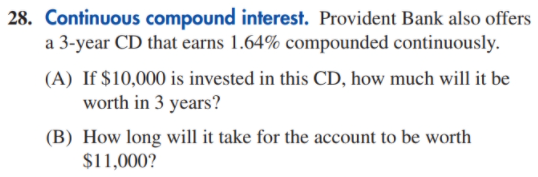
\includegraphics[width=0.75\linewidth]{10-1-28}
\end{center}
(A) Using $A = Pe^{rt}$.
\begin{align*}
	A &= 10000e^{.0164(3)} \\
	&=\$10504.30
\end{align*}
(B) Starting with $A = Pe^{rt}$.
\begin{align*}
	A/P &= e^{rt} \\
	\ln(A/P)&=rt \\
	t &= \frac{1}{r} \ln(\frac{A}{P}) \\
	&= \frac{1}{.0164} \ln(\frac{11000}{10000}) \\
	&\approx 5.8 \text{ years}
\end{align*}

\subsubsection*{Homework}
27, 29, 31,35, 43


\cleardoublepage
\subsection{Section 10.2: Derivative of Exponential and Logarithm}
\subsubsection*{Goals}
\begin{itemize}
	\item Understand these inverse functions, $\ln(e^x) = x$ and $e^{\ln(x)} = x$.
	\item Recall and use the derivatives for $\ln(x)$ and $e^x$.
\end{itemize}
\subsubsection*{Detail}
Inverses
\begin{center}
	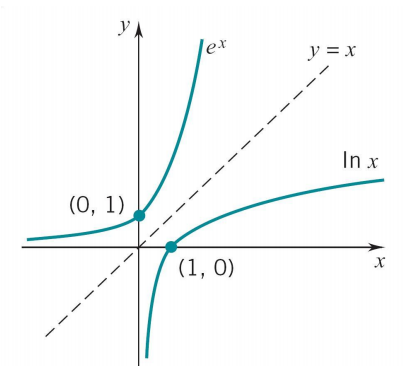
\includegraphics[width=0.5\linewidth]{10-2-1}
\end{center}
\begin{align*}
	&\ln(e^x) = x & & \text{and} & &e^{\ln(x)} = x 
\end{align*}
Derivatives
\begin{align*}
	&\frac{d}{dx}e^x =  e^x & &(\text{for all } x) \\\\
	&\frac{d}{dx}\ln(x) =  \frac{1}{x} & &(\text{for } x>0)
\end{align*}
Logarithm rules
\begin{align*}
	&\log(xy) = \log(x) + \log(y) & &\log(x/y)=\log(x)-\log(y) \\
	&\log(x^y)= y\log(x)	& &\log(1)=0
\end{align*}

\subsubsection*{Examples}
Find the derivatives
\\
(A)
\begin{align*}
	f(x) &= e^x + ln(x^2) + \frac{3}{5\sqrt{x}} \\\\
	&= e^x + 2ln(x) + \frac{3}{5}x^{-1/2} \\
	f'(x) &= e^x +(2)\frac{1}{x} + \left( \frac{3}{5}\right) \frac{-1}{2} x^{-3/2} \\
	&= e^x +\frac{2}{x} - \left( \frac{3}{10}\right) x^{-3/2}
\end{align*}
(B) 
\begin{align*}
	f(x) &= 3e^x + ln(x/5) + ln(e^{10x}) \\ \\
	&= 3e^x + ln(x/5) + ln(e^{10x}) \\
	&= 3e^x + ln(x) - ln(5 )+ 10x \\
	f'(x) &= 3e^x + \frac{1}{x} + 10
\end{align*}

\subsubsection*{Homework}
13-31 all



\cleardoublepage
\subsection{Section 10.3: Product and Quotient Rules}
Product Rule is:
\begin{align*}
	&\text{Given: } & &F(x) \text{ with derivative } F'(x) \\
	& & &S(x) \text{ with derivative } S'(x) \\
	&\text{and } & &f(x) = F(x)S(x) \\
	&\text{then }\\
	& & &f'(x) = F'(x)S(x) + F(x)S'(x)
\end{align*}
Quotient Rule is:
\begin{align*}
	&\text{Given: } & &P(x) \text{ with derivative } P'(x) \\
	& & &Q(x) \text{ with derivative } Q'(x) \\
	&\text{and } & &f(x) = \frac{P(x)}{Q(x)} \\
	&\text{then }\\
	& & &f'(x) = \frac{P'(x)Q(x) - P(x)Q'(x)}{(Q(x))^2}
\end{align*}

\subsubsection*{Examples}
\begin{align*}
	&\text{(48)} &y &= (x^3 + 2x^2)(3x-1) \\
	&			&y' &= (3x^2 + 4x)(3x -1) + (x^3 + 2x^2)(3) \\
	&			&    &= 9x^3 + 12x^2 - 3x^2 -4x + 3x^3 +6x^2 \\
	&			&    &= 12x^3 + 15x^2 - 4x\\\\
	&\text{(54)} &\frac{d}{dw} \frac{w^4 - w^3}{3w-1}&= \frac{(4w^3 - 3w^2)(3w-1) - (w^4 - w^3)(3)}{(3w-1)^2} \\
	&	&		&= \frac{12w^4- 4w^3 - 9w^3 + 3w^2 - 3w^4 + 3w^3}{(3w-1)^2} \\
	&	&		&=\frac{9w^4- 10w^3 + 3w^2 }{(3w-1)^2} \\
	&	&		&=\frac{w^2(9w^2- 10w + 3) }{(3w-1)^2} \\
\end{align*}



\cleardoublepage






\end{document}
